\begin{XeClass}{MD5MD5CRC32FileChecksum}
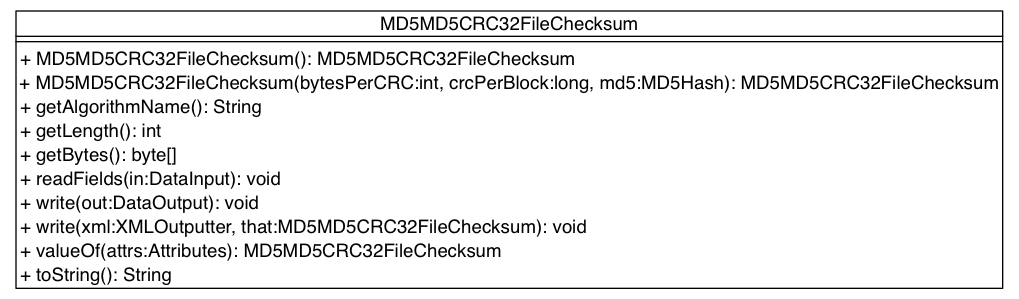
\includegraphics[width=10cm]{cdig/MD5MD5CRC32FileChecksum.png}
     
 MD5 of MD5 of CRC32.
 MD5MD5CRC32FileChecksum继承自FileChecksum,
 MD5加密并用CRC32校验和校验结果,
 定义三个私有成员变量,bytesPerCRC,crcPerBlock和md5,
 声明有静态成员常量LENGTH = MD5Hash.MD5_LEN + (Integer.SIZE + Long.SIZE)/Byte.SIZE

    \begin{XeMethod}{\XePublic}{MD5MD5CRC32FileChecksum}{MD5MD5CRC32FileChecksum}
         
 构造函数对三个成员变量初始化
 bytesPerCRC = 0
 crcPerBlock = 0
 md5 = null

    \end{XeMethod}

    \begin{XeMethod}{\XePublic}{MD5MD5CRC32FileChecksum}{MD5MD5CRC32FileChecksum}
         

    \end{XeMethod}

    \begin{XeMethod}{\XePublic}{String}{getAlgorithmName}
         
 返回算法名称

    \end{XeMethod}

    \begin{XeMethod}{\XePublic}{int}{getLength}
         
 返回静态常量LENGTH

    \end{XeMethod}

    \begin{XeMethod}{\XePublic}{byte[]}{getBytes}
         
 调用WritableUtils返回一个byte数组

    \end{XeMethod}

    \begin{XeMethod}{\XePublic}{void}{readFields}
         
 通过从数据输入流中读入bytesPerCRC,crcPerBlock,md5的值

    \end{XeMethod}

    \begin{XeMethod}{\XePublic}{void}{write}
         
 将bytesPerCRC,crcPerBlock,md5的值写入到数据输出流中

    \end{XeMethod}

    \begin{XeMethod}{\XePublic}{void}{write}
         
 将MD5MD5CRC32FileChecksum对象that的bytesPerCRC,crcPerBlock,md5的值写入到XML文件中

    \end{XeMethod}

    \begin{XeMethod}{\XePublic}{MD5MD5CRC32FileChecksum}{valueOf}
         
 静态方法valueOf,通过外部实体attrs获得bytesPerCRC,crcPerBlock和md5的值
 当外部实体未被找到时候抛出异常,并返回MD5MD5CRC32FileChecksum对象

    \end{XeMethod}

    \begin{XeMethod}{\XePublic}{String}{toString}
         
 返回算法名称+ ":" + md5

    \end{XeMethod}

\end{XeClass}
